\documentclass[conference]{IEEEtran}
\usepackage{graphicx}
\usepackage{amsfonts}
\usepackage{amssymb}
%\usepackage[spanish]{babel}
\usepackage{verbatim}
\usepackage{amsbsy}
\usepackage{algorithm}
\usepackage{algorithmic}
\usepackage[T1]{fontenc}		%Previene errores en el encoding
\usepackage[utf8]{inputenc}		%para identificar acentos(encoding)
\usepackage{hyperref} %para url´s 
% correct bad hyphenation here
\usepackage{placeins} %para el FloatBarrier
\hyphenation{optical networks semiconductor IEEEtran}
%decimalpoint %decimales
%newtheorem{definition}{Definicion}[section]
%newtheorem{theorem}{Teorema}[section]
%newtheorem{lemma}{Lema}[section]

\begin{document}

% paper title
\title{An application of the Ncut algorithm, with an open-source implementation (in the R environment).  }


% author names and affiliations
% use a multiple column layout for up to three different
% affiliations
\author{\IEEEauthorblockN{J. Antonio Garcia Ramirez}
\IEEEauthorblockA{Centro de Investigacion en Matematicas. Unidad Monterrey\\
jose.ramirez@cimat.mx}
}



% make the title area
\maketitle

\begin{abstract}
Although the analysis of data is a task that has gained the interest of the statistical community in recent years and whose familiarity with the statistical computing environment, they encourage the current statistical community (to students and teachers of the area) to complete statistical analysis reproducible by means of the tool R.
However for years there has been a gap between the calculation of matrices on a large scale and the term "big data", in this work the Normalized Cut algorithm for images is applied. Despite the expected, the R environment to do image analysis is poorly, in comparison with other computing platforms such as the Python language or with specialized software such as OpenCV \cite {OpenCV}. \\
Being well known the absence of such function, in this work we share an implementation of the Normalized Cut algorithm in the R environment with extensions to programs and processes performed in C ++, to provide the user with a friendly interface in R to segment images. The article concludes by evaluating the current implementation and looking for ways to generalize the implementation for a large scale context and reuse the developed code.

\textit{Key words: Normaliced Cut, image segmentation, Lanczos algorithm, eigenvalues and eigenvectors, graphs, similarity matrix, R (the statistical computing environment), open source, large scale and big data.}\end{abstract}

\IEEEpeerreviewmaketitle


\section{Introduction and motivation}



The statistical recognition of patterns, and in particular the analysis of images, is a stimulating field of study where statistics and computer science coexist. In recent years the environment of statistical computing and programming language R \cite{R} has increased its presence in statistical analysis and is even used in big data contexts, on the other hand, image analysis is an area that continues to motivate investigation.\\
As a counterpoint to what is expected, since image analysis uses different statistical learning techniques (both supervised and non-supervised), the R environment has few tools for image analysis, as can be seen when reviewing the entry of 'MedicalImaging' in its Task View, in front of other specialized tools such as OpenCV \cite{OpenCV}. On the other hand, there are scientific computing environments that integrate some tools to analyze images, but their capacities are reflected in their commercial price, for example MatLab \cite{MatLab}. \\
%%%%%
The above, together with the fact that image segmentation is a final objective and sometimes only an intermediate step in other investigations, in this work an image segmentation application is developed using the Normalized Cut algorithm, which we will refer to in the following as \textit{Ncut}. In order to provide users and developers of the R language with an implementation of the \textit{Ncut} algorithm (which does not exist in OpenCV and other scientific computing environments), two programs were coded; each contains a file with extension .R that determines it as an R language code as well as a file with extension .cpp that is a C ++ language code that uses stable C ++ language libraries to perform calculations and optimal storage of matrices;
one for grayscale images and one for RGB images available in the github author's personal \cite{github}  \url{https://github.com/fou-foo/MCE/tree/master/Second/AnalisisNumericoYOptimizacion/Miniproyecto} respectively the files are ''W\_float.cpp'' and ''mini\_cut\_float.R'' for grayscale images and ''W\_RGB\_float.cpp'' and ''mini\_Ncut\_RGB\_float.R'' for images on RGB channels (which is easily adaptable to images with more channels). Details on implementation are discussed in the last subsection of section ''II. Workflow ''of this report. \\
With the above, an easy-to-use open-source tool is provided, particularly in the R environment, although the .cpp code can be exported to other computing environments, for the Ncut algorithm, which provides the basis for future statistical computing developments. The product developed allowed to segment a set of images from the personal profile of the author of the Facebook \cite{Facebook} platform, whose results are reported in this work. \\
The organization of the present work is as follows: in the section 'II. Workflow" is explained in a general way in which the Ncut algorithm that was used in this work consists, as well as its relation with the Lanczos algorithm, later the implementation of the algorithm is detailed so that it is easy to use in the R environment.In the section ''III. RELATED WORKS'' we report the research carried out on the lack of implementations of both the Ncut algorithm and the Lanczos algorithm in different architectures (which makes the need for an own implementation tangible) such as tools dedicated to the big data context (such as Apache Hadoop \cite{Hadoop} and Apache Spark \cite{Spark}) where the author sees an area of opportunity for massive image analysis, on the other hand, in large-scale matrices there are implementations in MPI such as ScaLAPACK \cite{ScaLAPACK} of the Lanczos algorithm, however, they do not implement higher-level routines such as Ncut. We conclude this section by commenting on tools that we consider medium-term to be useful for large-scale scientific computing such as the programming language Elixir \cite{Elixir}. \\
Then in the section "IV. Experiments and Results" are shown (and in some images are detailed) the results of the image segmentation realized with the own implementation. The section concludes with the benefits and limitations of the implementation to obtain a "good" image segmentation. Later in the section "V. Conclusions" we summarize the discoveries learned and evaluate the methodology used. Finally, the "Appendix" section proposes future works of improvement of the implementation, within the open-source context, to segment images of greater resolution and size to those addressed in this work, as well as the possible extension to other statistical learning techniques with the purpose of reusing the code already developed and future. \\
\section{WORKFLOW}
\subsection{On the problem of segmenting images and the focus of Ncut}
The problem of segmenting an image (considering the values that each pixel can have in different channels) is usually formulated in mathematical terms in the following way: given an image whose set of pixels we call $ V $, it is sought to partition $ V $ in disjoint sets $ V_1, V_2, ... V_m $ where some measure of homogeneity (ie of similarity) between the pixels of each $ V_i $ is high while the same measure through different set $ V_i $, $ V_j $ is low. \\
Although the previous measure of similarity responds to the importance of visual, spatial and grouping perceptions, it must be shared in nearby pixels. In view of the fact that the set of all possible partitions of a set $ V $ is too large and grows exponentially as a function of the cardinality of $ V $, in fact, this is the definition of the Stirling numbers of the second type, it arises the question How to choose the "correct" partition? There are generally two ways to approach the problem: the first is to pay attention to low levels of coherence between brightness, color and texture in each pixel, however this approach tends to produce hierarchical segmentations where the larger hierarchies respond to groups and the smaller ones to individual pixels, in practice can be done with computationally costly algorithms such as the popular 'single' and 'ward' that produce dendograms. In contrast, the second approach to dealing with the problem is the one shared by Ncut, which is a downward focus, meaning that it first pays attention in larger areas and then looks at the details, following the analogy of \cite{Ncut} ''as a painter first marks the large areas and then fills the details''. \\
Following the ideas of \cite{Ncut}, the problem of image segmentation consists of two points:

\begin{enumerate}
\item What is the precise criterion for a good partition? That is, define the similarity between elements of $ V $
\item How can such that partition be computed efficiently?
\end{enumerate}  
Briefly, the approach suggested by \cite{Ncut}, to partition an image is to consider the pixels of a $ V $ image as the vertices of a graph $ G = (V, E) $ and form a partition in two sets $ A $ and $ B $ such that $ A \cup B = V $, $ A \cap B = \emptyset $, simply removing edges that connect both parts. The degree of dissimilarity between $ A $ and $ B $ can be calculated as the total weight of the edges that were removed, in graph theory this is called \textit{cut}:
\[
cut (A, B) = \sum_{u \in A, v \in B} w (u, v)
\]
Finding the minimum cut is a well-studied problem, even at the undergraduate level of careers such as applied mathematics or computer science, and there are efficient algorithms to solve it. \\
On the other hand \cite{Ncut} proposes the following measure of dissociation between groups, \textit{Normalized cut}:
\[
Ncut (A, B) = \frac {cut (A, B)} {assoc (A, V)} + \frac {cut (A, B)} {assoc (B, V)}
\]
Where $ assoc (A, V) = \ sum_ {u \ in A, t \ in V} w (u, t) $ corresponds to the total connections of the nodes in the set $ A $ to all nodes in the graph and $ assoc (B, V) $ is defined similarly. A fundamental result of \ cite {Ncut} is that minimizing dissociation through groups, ie the measure $ Ncut $, is equivalent to maximizing the association within each group and that both conditions can be satisfied simultaneously.
\subsection{Mathematical and computational aspects}
As commented in \cite{Ncut} finding the optimal $ Ncut $ exactly is an NP-complete problem (whose elegant proof is found in appendix A of the same paper \cite{Ncut} and is attributed to Papadimitrou). However, the authors of \cite{Ncut} prove that relax the conditions to the continuous domain an approximate solution to the discrete problem can be found efficiently and after defining notation and with a little algebra the authors of the paper show that this approximate solution to the minimization of $ Ncut $ corresponds to:
\begin{equation}
\min_{\boldsymbol{x}}Ncut(\boldsymbol{x}) = \min_{\boldsymbol{y}} \frac{\boldsymbol{y}^t(D-W)\boldsymbol{y}}{\boldsymbol{y}^tD\boldsymbol{y}}
\end{equation}
Where $ \boldsymbol {x} $ is an indicator vector with 1 in the ith position if the i-th pixel is in $ A $ and -1 in all other $ | V | -1 $ entries, $ D = diag (d_1, d_2, ..., d_ {| V |}) $ is the diagonal matrix where $ d_i = \sum_j w (i, j) $, $ W $ is simply the weights matrix of edges is $ W (i, j) = w_{ij} $, and finally $ \boldsymbol {y} $ is the vector where each entry $ i \in \{1, -b \} $ with $ b = \frac {\sum_ {x_i> 0} d_i} {\sum_ {x_i <0} d_i} $ and $ \boldsymbol {y} D \boldsymbol {1} = 0 $ where $ \boldsymbol {1} $ is a vector of dimension $ | V | $ with 1's on all your tickets. \\
From the above the authors of \cite{Ncut} recognize that (1) corresponds to the quotient of Rayleigh \cite{MatrixC}. Relaxing the condition that $  \boldsymbol {y} $
taking real values (1) is minimized by solving the generalized eigenvalues problem:
\begin{equation}
(D-W)y = \lambda D y
\end{equation}
As shown in \cite{Ncut} (2) it is equivalent to the standard eigenvalues problem
\begin{equation}
D^{-1/2}(D-W)D^{-1/2}z = \lambda z
\end{equation}
Where $ z = D ^ {1/2} and $. An interesting property of (3) is that $ z_0 = D ^ {1/2} \boldsymbol {1} $ is an eigenvector associated with the eigenvalue 0, moreover $ D ^ {-1/2} (D-W) D ^ {- 1/2} $ is symmetric and semi positive definite, so $ z_0 $ is the eigenvector associated with the smallest eigenvalue and by a specific result of the courses of linear algebra, the eigenvectors of a matrix are perpendicular so the eigenvector associated with second smallest eigenvalue of (3) is perpendicular to $ z_0 $. Then, the eigenvector associated with the second smallest eigenvalue of (3) is the actual solution of (2). \\
Both in the application made in the set of images and in the implementation, explicitly (3) is used to find the desired partition by means of the corresponding eigenvalues and eigenvectors. As stated in \cite{Ncut} there are several peculiarities about the use of the previous result. An image can be segmented using the $ k $ eigenvalues, and their corresponding eigenvectors smallest which is computationally expensive by the dimensions of $ W $ so if the original image is of size $ h \times w $ then $ W $ has dimensions $ (h \times w) \times (h \times w) $, so we can start from finding the first solution of (3) and perform the same procedure on each set $ A $ and $ B $ ( which is computationally more efficient, since the matrix $W $ has been previously calculated). In our application, our approach consisted in segmenting using the eigenvector associated with the second smallest eigenvalue of (3) to identify two groups, and this was also considered in conjunction with the eigenvector associated with the third smallest eigenvalue of (3) to segment in 3 sets, in our workflow, by obtaining the two aforementioned eigenvectors, we apply the kmeans algorithm to the vector inputs to have more defined groups. It is important to mention that in view of the nature of the algorithm  \textit{Ncut}  the preprocessing phase of the images with which it was worked does not include any filter on the original image. \\
Then the grouping algorithm used in our application consists of: \\
\begin{enumerate}
\item Given an image of size $h \times w$ with $n$ channels, considered as a graph $G = (V, E)$, construct the matrix of weights $W$ connecting two nodes with a measure of similarity between pairs of nodes For which we choose a Gaussian kernel defined as
\[
W_{ij}= e^{-||x_{(i)}-x_{(j)}||^2_2/2\sigma^2_I}e^{-||x_{(i)}-x_{(j)}||^2_2/2\sigma_x^2}
\]
If $ || x _ {(i)} - x _ {(j)} || _2 ^ 2 <r ^ 2 $ and 0 otherwise where $ x_ {(i)} $ is the i-th pixel of the image . In our experiments we fix $ \sigma_x ^ 2 = 10 $, $ \sigma_I ^ 2 = 0.05 $ and following the recommendation of \cite {Ncut} we set $ r = \left \lfloor
 \sqrt {\frac {(h \times w) -1} {2} * 0.1} \right \rfloor +1 $, that is, we consider that each pixel is connected to the most with $ r ^ 2 $ pixels around him in the metric $ L_2 $. \\
\item Solve (3) and save the eigenvectors associated with the second and third smallest own values
\item First use the eigenvector associated with the second smallest eigenvalue and apply its kmeans entries, then use the two eigenvectors mentioned in the previous point and also use kmeans on its inputs to partition the image into two and three sets respectively.
\end{enumerate}
In general, solving the problem of eigenvalues for all eigenvalues requires $ O (p ^ 3) $ operations, where $ p $ is the number of pixels in the image (in our notation $ p = h \times w $ ), which makes $ Ncut $ impractical for large image segmentation, however in our experiments we manage images with up to 19,200 pixels (138 pixels on each side for square images), but for our particular application we have aspects that favor computation : first our matrix $ W $ is symmetric (which is a consequence of the symmetry of the kernel used), semi positive definite and sparse (in view of the construction of $ r $) and we only need the eigenvectors associated with the three eigenvalues smaller, as mentioned in \cite{Ncut} the accuracy of the eigenvalues is low because as we could experimentally prove the distribution of the entries of the eigenvectors mentioned makes it clear that knowing the sign corresponding to the entry of the own vector is enough to classify in addition to the comments of \cite{Ncut} experimentally we found that the calculation of $ W $ only requires operations between numbers of floating arithmetic of the type \textit {float } in C ++ in a 64-bit architecture. The aforementioned properties are fully exploited by the Lanczos method, which has a complexity of $ 0 (mp) + O (mM (p)) $ \cite{MatrixC} where $ m $ is the maximum number of calculations of the type matrix-vector (with sparse matrices) and $ M (p) $ is the cost of matrix-vector multiplication, as we work with sparse matrices the complexity of $ M (p) $ is $ O (p) $. \ \ 
We summarize the workflow that was followed to segment images using Ncut in figure 1. Where the blue color indicates that this task was used using the R language and the orange color indicates that the task was done through the C ++ language. In particular, the preprocessing of the second step consisted of resizing the images so that the number of pixels in them did not exceed 19,200 in the necessary cases, which is done by means of a closer neighbor interpolation, with which image information is lost. original but makes segmentation feasible in this new size. In addition to normalizing the values of the pixels in each channel, that is to say that in each channel for each pixel value is subtracted with the minimum value found in the channel is left and the result was divided among the range of the original channel (difference between the maximum value and the minimum). 
\begin{figure}[htbp]
\center{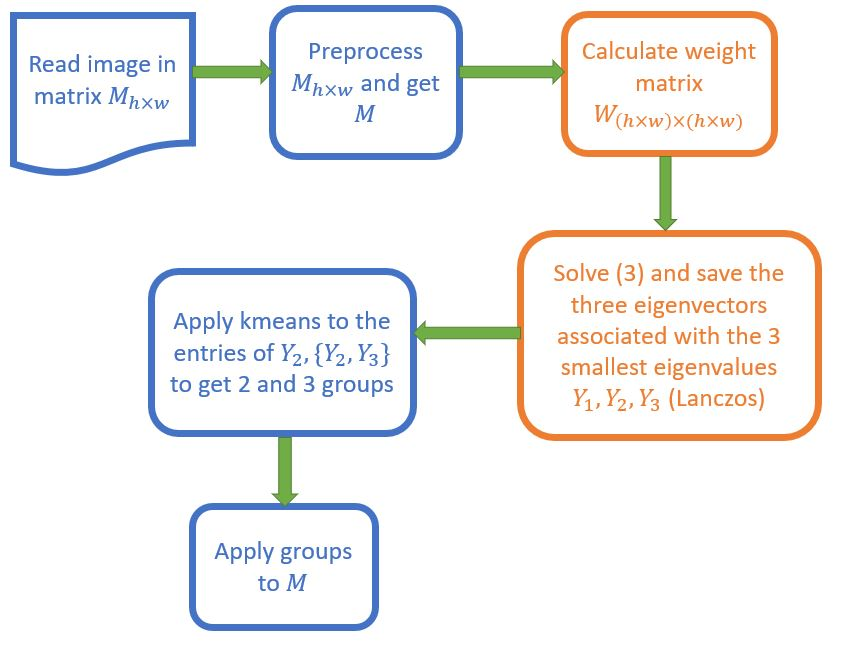
\includegraphics[width=7cm]{workflow_english.JPG}}
\caption{Workflow to segment images}
\label{workflow}
\end{figure}\\
\subsection{Details of the implementation (in particular in the R language)}
The R programming language in particular has challenges in the application of the \textit{Ncut} algorithm due to the following reasons:
\begin{enumerate}
\item The representation of the images and in general of the floating point numbers correspond to the standard of \textit {double} of the C ++ language
\item R loads all the objects with which you work in RAM.
\end{enumerate}
However the sparse matrices are easy to handle in the R. environment.\\
Following the diagram in figure 1, the disk reading was did with the package \textit{imager} \cite{imager} which represents the images as a 4-dimensional array where the first two dimensions correspond to the height and width of the image, and the fourth dimension corresponds to the channels available to the image. This 4-dimensional representation uses the type \textit{numeric} of R that corresponds to 64-bit C ++ data type \textit{double}. In cases where it is required to resize the image, it was done with the same package of R. \\
To counteract point (1) above, the calculation of the $ W $ matrix is done in C ++ by restricting the type of data between operations to the type \textit{float}, for which the Rcpp \cite{Rcpp} package is used and to store the matrices in a sparse matrix format, the RcppEigen \cite{RcppEigen} package is used, which allows to interact with the Eigen library of the C ++ language, so that the output of the C ++ code is an array $ W ^ * $ symmetric, positive semi-definite and of the sparse type that incorporates the necessary information to solve the problem of the eigenvalues of equation (3).
In particular, the program that segments images with more than one channel uses the RcppArmadillo \cite{RcppArmadillo} package, which has an interface to use the C ++ Armadillo linear algebra library, to use 3-dimensional arrays (in this point is important to mention that the real implementation requires changes to the header of the file \textit{RcppArmadillo.h}, increase the line ''\#include <RcppEigen.h>'' as the default installation and the process of \textit {attach} (innate of the R language) conflicts the headers \textit {RcppEigen.h} and \textit {RcppArmadillo.h} as both refer to the \textit {Rcpp.h} header, however when add the mentioned line a single header includes a others in a single invocation and \textit {attached file}). \\
Up to this point we used the C ++ language for the calculation of $ W $, notably improving the execution time compared to doing it in R, besides saving memory space of 50 \% when using only the data type \textit {float } instead of \textit {double} \\
To counteract point (2) of the previous list, objects that are no longer required are explicitly removed from the environment and we explicitly called the garbage collector. The package for the fourth step uses a function of the Rspectra \cite{RSpectra} package, which is an interface to the Spectra library developed in C ++ similar to the ARPACK library (developed in Fortran), which refers to a C ++ implementation of the Lanczos method implicitly restarted and to obtain the smallest eigenvalues in the place of the large ones, which use the method of change around the zero in place explicitly, the matrix $ W ^ * $. \\
The fifth step that consists in applying kmeans on the eigenvectors obtained previously, was done with the implementation of the base kernel of R with 50 iterations and fixing the seed in both cases to provide reproducibility to the experiment, finally the application of the segmentation corresponds to a convolution of matrices between the original image, after having been resized if necessary, and the arrangement of the segmented pixels. In the case of images with three channels, this convolution maps by channel to the original value of the pixel to zero, or multiplies it by 0.5 or leaves it intact depending on which segment it belongs to.
\section{Related jobs}
In the previous section we detailed an implementation to segment images using the \textit {Ncut} algorithm that depends strongly on the implementation of the RSpectra \cite {RSpectra} package of the implicitly restarted Lanczos method, which, as we mentioned earlier, invokes an implementation in C ++ of its analog in Fortran of the classic ARPACK \cite {Arpack} library to solve the problem of finding the eigenvectors associated with the smallest eigenvalues of a positive and scattered semidefinite symmetric matrix. However, the current implementation is limited in terms of the size of the $ W $ matrix, which is why we resort to resizing the images in sizes approximately greater than $ 138 \times 138$. \\
In a large-scale context the ScaLAPACK \cite {ScaLAPACK} library implemented a routine that solves the problem of values and eigenvectors for the symmetric case (such as the one we attacked), however in a big data context there are friendly implementations, even with a API to the Python language (see \url {https://spark.apache.org/docs/2.3.0/mllib-dimensionality-reduction.html}), of the SVD decomposition (considering only the largest singular values ) whose implementation is detailed in \cite {MatrixSpark}, with this work (and its current implementation of the QR decomposition) or with the implementation of the inverse of a matrix in the Spark environment proposed in \cite {Sparkbased} makes it plausible to scale the problem and the segmentation of images using the \ textit {Ncut} algorithm, however, this requires a new data and computing architecture. \\
On the other hand we hope that programming languages that are born as functional and concurrent as Elixir \cite{Elixir} will develop robust libraries for scientific computing in the medium term, since today the language has a linear algebra library, without However, it is still in a state of development \cite {ElixirLib}, as we can see by noting that its implementation of the inverse of an 'inv' matrix uses Gaussian elimination and brute force.
\section{Experiments and results}
The current implementation we shared of the algorithm \textit {Ncut}, was applied to a set of images from the author's Facebook profile. The experiments are reported in the following Table I, making reference to each image with a number and the average time of the execution in the image. The experiments were performed on an Asus GL553VD machine with 8 GB of RAM (but due to the configuration of the Windows 10 operating system) it is only possible to fully use 6 of these 8 GB, with an Intel Core i7-7700HQ processor (with 8 logical cores) at a speed of 2.5GZ. \\
During the execution times, and part of the development, we were able to estimate the amount of RAM a PC requires to execute the current implementation of \textit {Ncut}, which is approximately 4 times the space required to store the array $ W $ , this because at some point it is required to have in memory two matrices additional to the $ W $ matrix of the same dimensions and same characteristics, in addition to the memory that the Lanzos implementation uses to be made.\begin{table}[h]
\begin{center}
\begin{tabular}{c|cccccc}
\hline  \begin{tabular}{@{}c@{}}Image's\\ number\\ and name \end{tabular}  &\begin{tabular}{@{}c@{}}Original\\size\end{tabular}& \begin{tabular}{@{}c@{}}Analyzed\\size\end{tabular} 
%(después de redimensionarla) 
& \begin{tabular}{@{}c@{}}Execution\\time\\ grayscale\\(mins)\end{tabular} & \begin{tabular}{@{}c@{}}Execution\\time\\ RGB\\(mins)\end{tabular} &  \begin{tabular}{@{}c@{}}Matrix\\size\\$W$\\(MB)\end{tabular}\\ \hline
1: Cell.jpg	     &100	$\times$ 69        & 100$\times$ 69 & 22.3 secs&	17.6 secs & 133.1\\
2: los\_amantes.jpg  &397 $\times$ 504     & 397$ \times$ 504   & 2.1 &2.4& 429.1\\
3: foo.jpg	&528 $\times$	528 &  132$\times$132	& 4.6&5.9 &855.2\\
4: guapa.jpg &970$\times$	720 & 100$\times$	180	&4.6& 4.9& 330.1\\
5: fer.jpg &533$\times$960 &100$\times$180 & 8.8 & 7.0 & 874\\
6: brindis.jpg	&1280$\times$960 & 160$\times$120 & 13.7 &7.1& 1000\\
7: foo\_clau.jpg &1280$\times$720&	104$\times$180 & 7.0& 8.1& 954.6\\
8: f002.jpg&960$\times$960&138 $\times$138& 16.9&8.9&1000\\
9: frascos.jpg&2048$\times$1152&180$\times$103&7.5&4.1&943.4\\
10: foo3.pjg&960$\times$960&138$\times$138&11.3&12.4&1000\\
%11: luis.jpg&2048$\times$1365&165$\times$110&3.8&10.2 &926.7\\
11: bicis.jpg&1280$\times$960& 160$\times$120&31.5&33.5&1000\\
%12: santa\_lucia.jpg&2048$\times$1152&182$\times$102&8.1&7.5&943.8\\
12: mariposa.jpg&2048$\times$1151&178$\times$100&5.9&3.3&863\\
13: filo\_liz.jpg&2048$\times$1152& 182$\times$102&7.9&7.0&943.8\\
14: marco.jpg&2048$\times$1365& 166$\times$110&5.4&4.7&933\\
\hline
\end{tabular}
\caption{Summary of the execution of the algorithm \textit {Ncut} in the set of sample images. Note that from image 2 all the images were resized.}
\label{tresultados}
\end{center}
\end{table}
\FloatBarrier
Figure 2 (from top to bottom) shows the results obtained when selecting images 1 to 5 using the two sets of channels (grayscale and RGB) after being resized to the sizes described in table I. It is interesting to note that the results are ideal for images 1 and 5, on the other hand, for images 3 and 4 they can be identified by themselves, however, in image 2 as it is a photograph of a pencil, the clamps that hold up are easily identified the sketch and it is not until the segmentation with two eigenvectors (right) that is identified as the whole sketch as a single differential set of the tweezers. \\
In figure 3 (from top to bottom) the results obtained by segmenting the images 6 to 10 using analogously notation to figure 2 are shown. It is interesting to note that the results are consistent when recognizing people from the background, for example figure 10 and 8 (where the person is detected even in the segmentation that uses only an own vector and achieving greater detail when using more components) however in image 6 the segmentation in RGB is only able to identify the clothes of the person in green . When viewing the image 9 we noticed that in particular the implementation is delicate recognizing glass objects however it distinguishes well other materials such as plastic. In particular of the results of Figure 6 and 7 we can see that the light conditions affect the performance of the implementation which suggests an improvement in the preprocessing for future work. \\
\begin{figure}[htbp]
\center{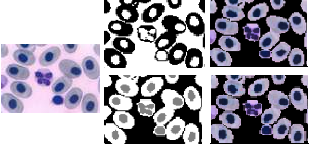
\includegraphics[width=5.0cm]{res_cel.png}}
\center{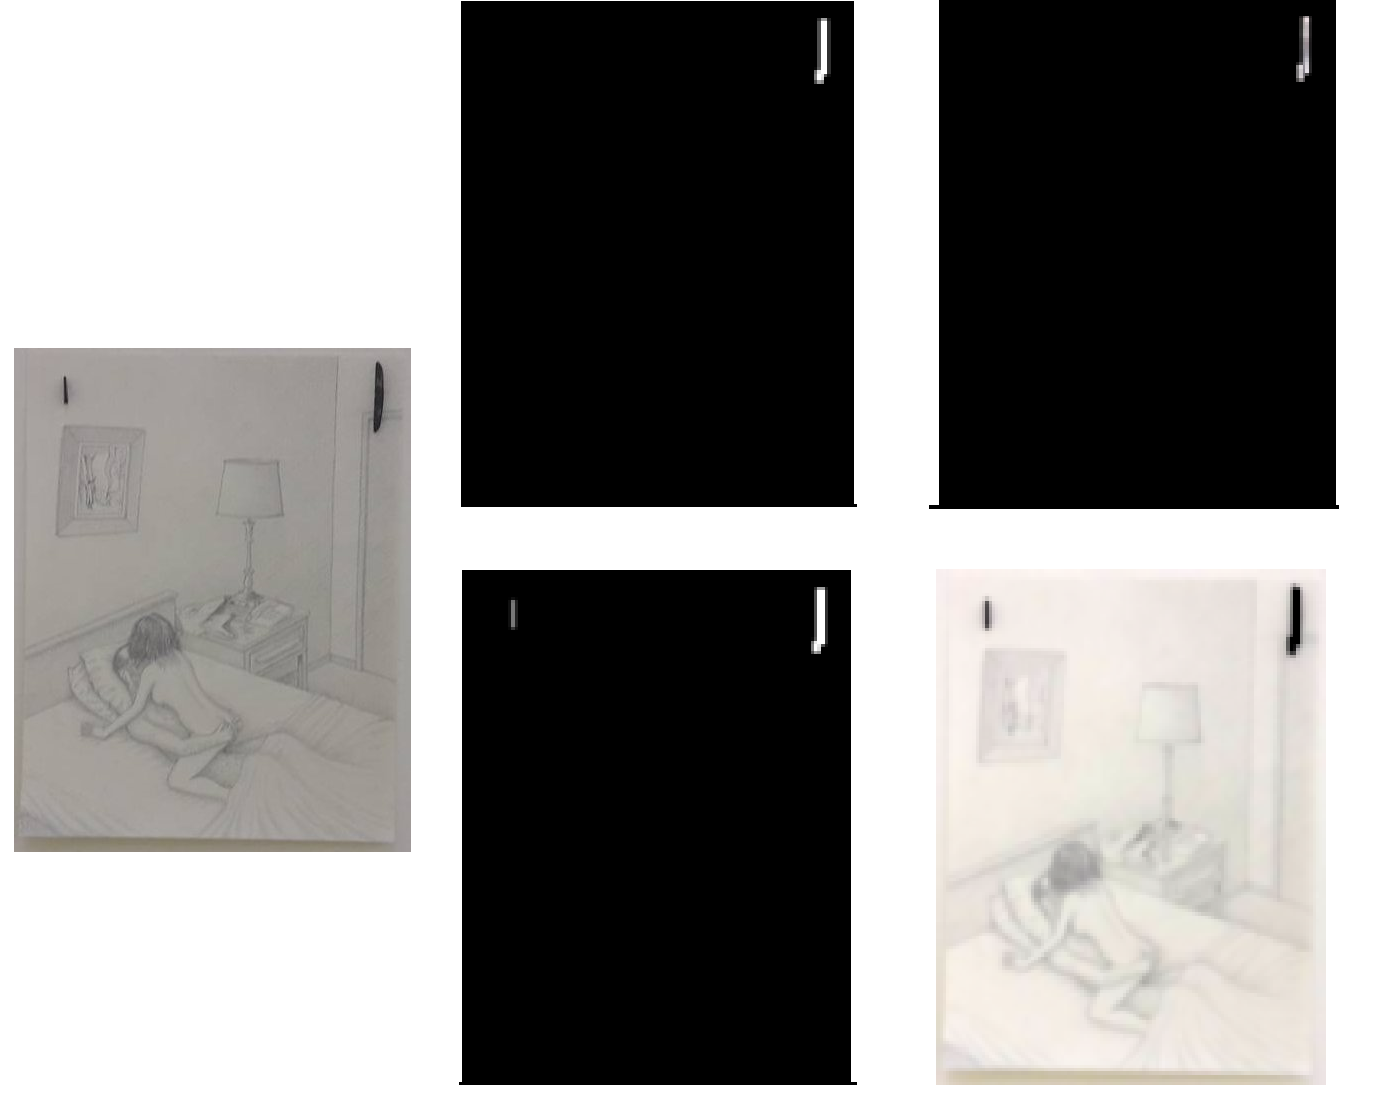
\includegraphics[width=5.5cm]{res_los_amantes.png}}
\center{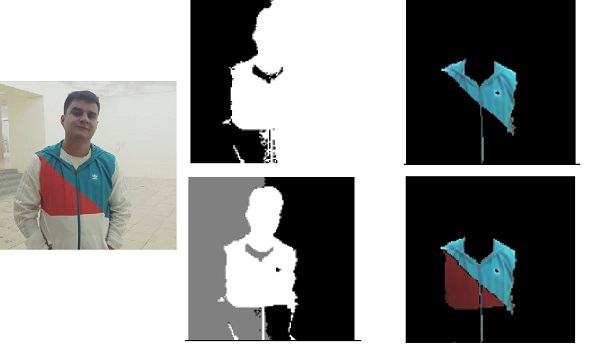
\includegraphics[width=5.0cm]{res_foo.jpg}}
\center{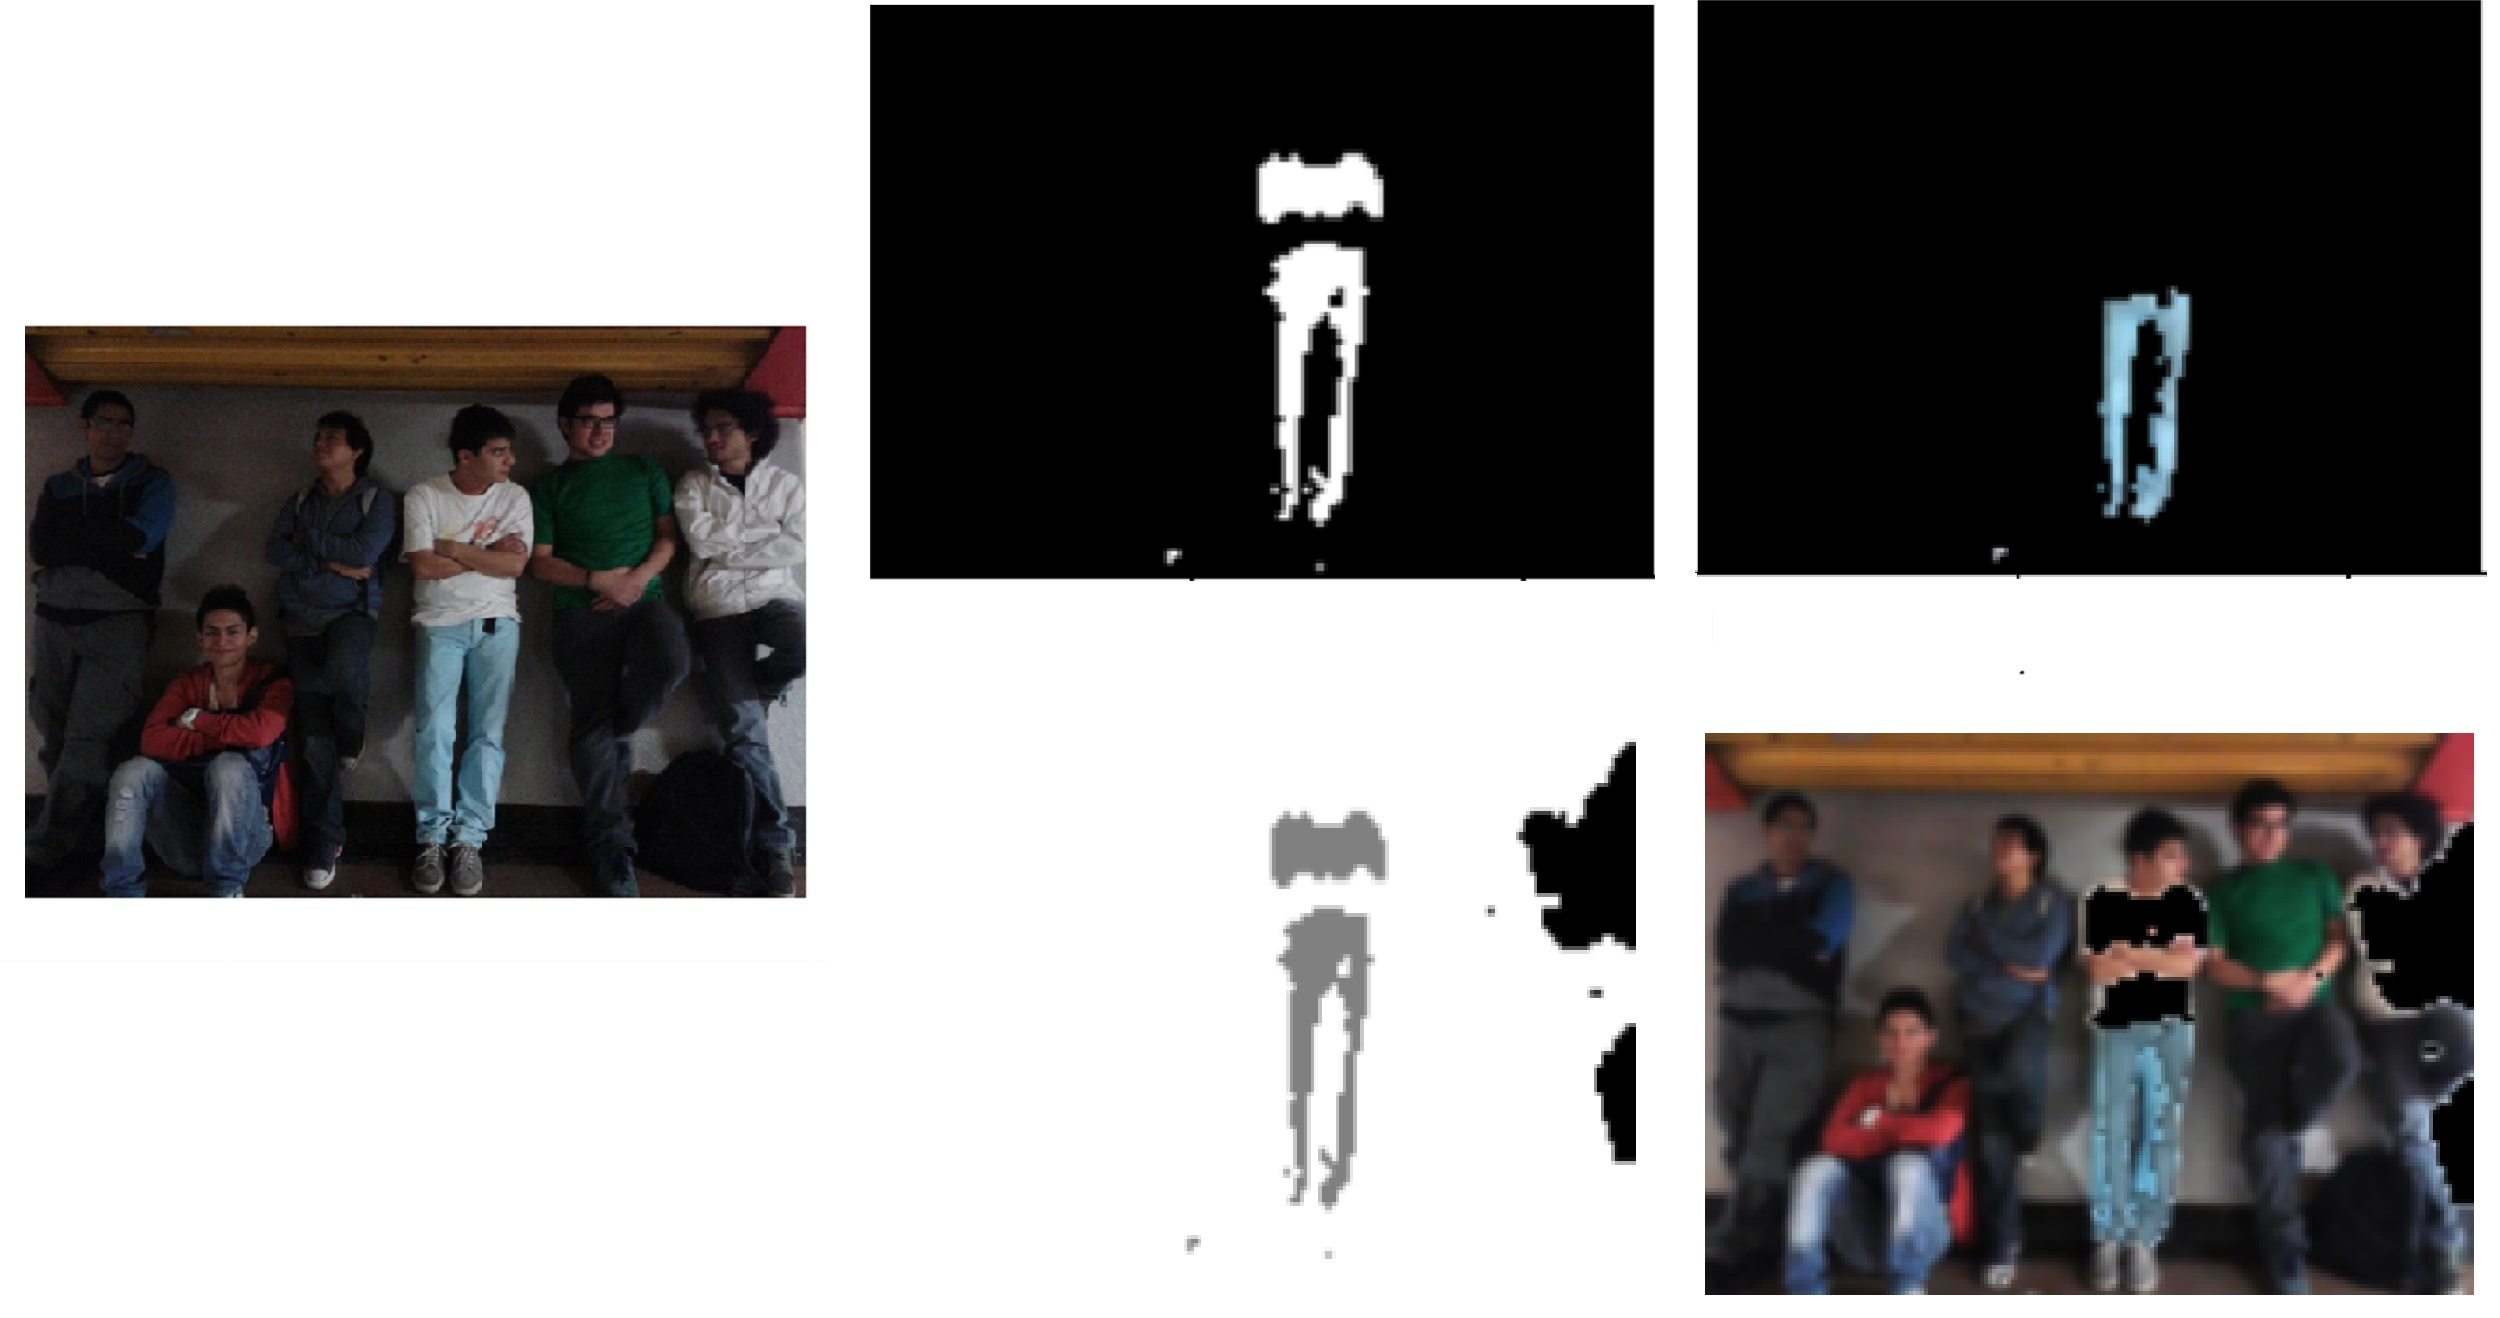
\includegraphics[width=5.0cm]{res_guapa.jpg}}
\center{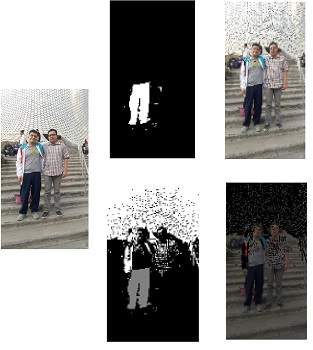
\includegraphics[width=5.0cm]{res_fer.jpg}}
\caption{Results of the segmentation of images 1 to 5, original image (left), segmentation obtained using the eigenvector associated with the second smallest eigenvalue in grayscale and RGB (center and right above) and segmentation obtained using the associated eigenvectors to the second and third smallest eigenvalue in grayscale and RGB (middle and bottom right).}
\label{res1}
\end{figure}
\begin{figure}[htbp]
\center{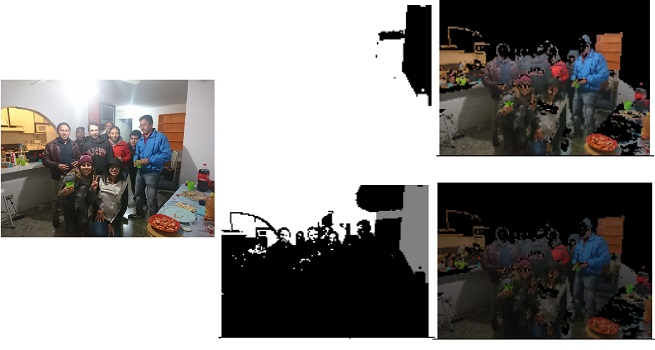
\includegraphics[width=6.3cm]{res_brindis.jpg}}
\center{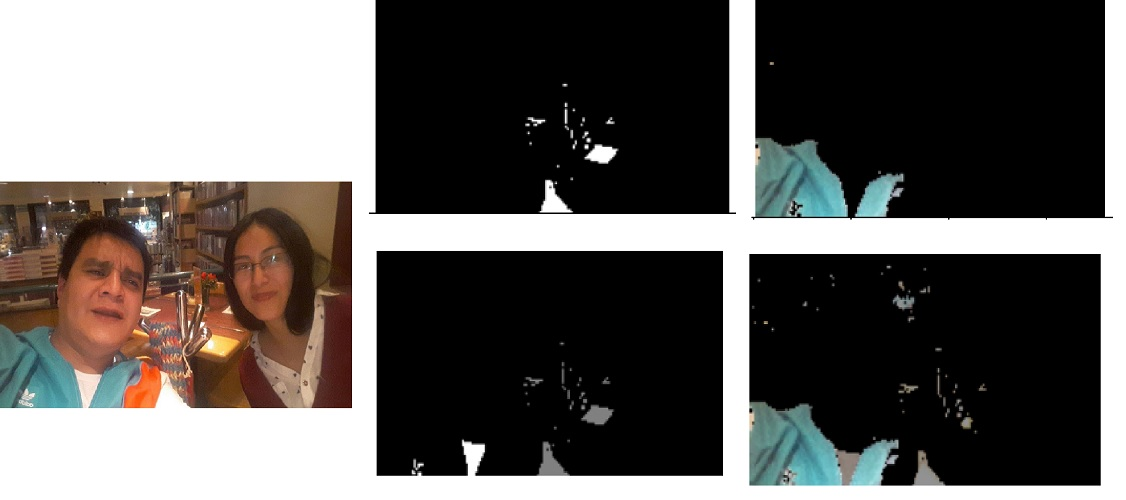
\includegraphics[width=6.3cm]{res_foo_clau.jpg}}
\center{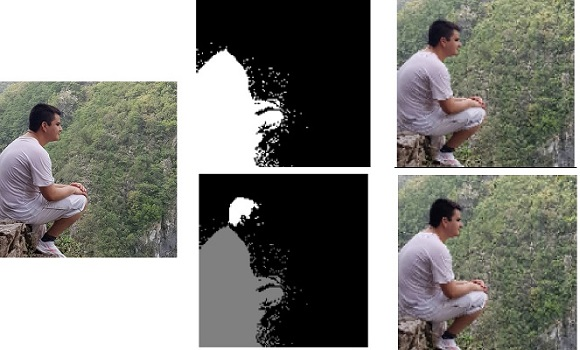
\includegraphics[width=6.3cm]{res_foo2.jpg}}
\center{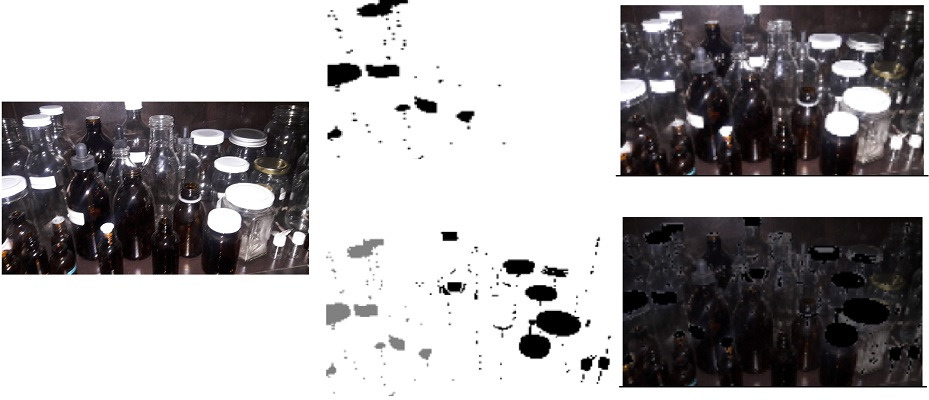
\includegraphics[width=6.3cm]{res_frascos.jpg}}
\center{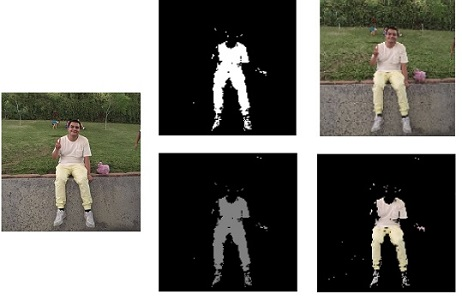
\includegraphics[width=6.3cm]{res_foo3.jpg}}
\caption{Results of the segmentation of images 11 to 14, original image (left), segmentation obtained using the eigenvector associated with the second smallest eigenvalue in grayscale and RGB (center and right above) and segmentation obtained using the associated eigenvectors to the second and third smallest value in grayscale and RGB (middle and bottom right).}
\label{res2}
\end{figure}
\FloatBarrier
\newpage
In figure 4 (from top to bottom) the results obtained through the images 11 to 14 are shown using analogously to figure 2. From the previous set of images we conclude: on the one hand, the image 11 shows that the information provided by the RGB channels is valuable to identify people from the background with a single eigenvector, in counterpoint the images 12 and 13 achieve greater performance in the gray scale (although the image of the butterfly in the RGB channels is easily distinguished). Finally, the image 14 is another sketch, but unlike the image 2, this is a photograph, where we see that the segmentation with the channels in the gray scale achieved a better performance when identifying the body however, this could be due to to causes of lighting at the time of taking the photograph.
\begin{figure}[htbp]
\center{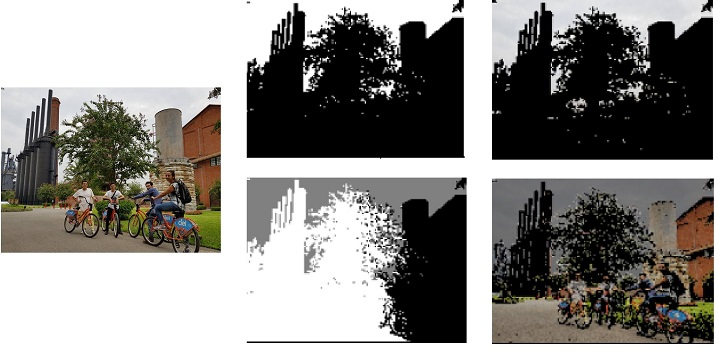
\includegraphics[width=6.65cm]{res_bicis.jpg}}
\center{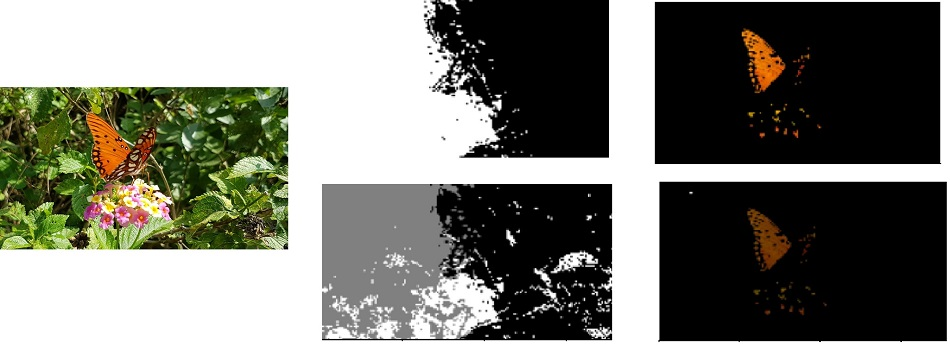
\includegraphics[width=6.6cm]{res_mariposa.jpg}}
\center{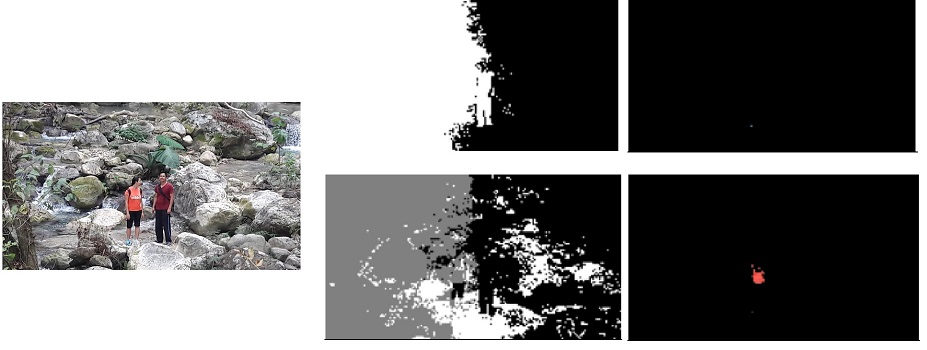
\includegraphics[width=6.6cm]{res_filo_liz.jpg}}
\center{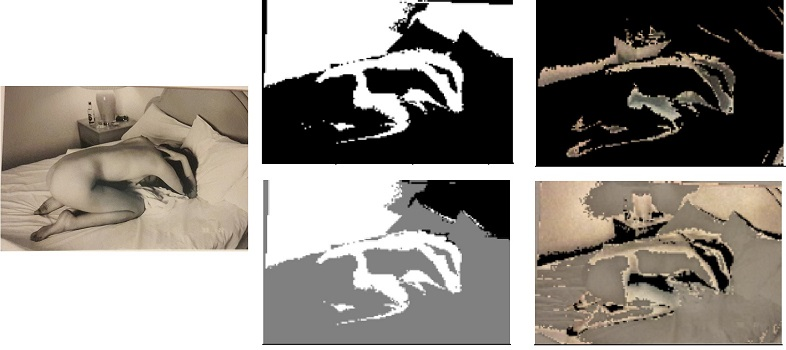
\includegraphics[width=6.65cm]{res_marco.jpg}}
\caption{Results of the segmentation of images 6 to 10, original image (left), segmentation obtained using the eigenvector associated with the second smallest eigenvalue in grayscale and RGB (center and right above) and segmentation obtained using the associated eigenvectors to the second and third eigenvalue smaller in gray scale and RGB (center and right below).}
\label{res2}
\end{figure}
\FloatBarrier
\newpage

\section{Conclusions}
In general terms, what has been learned in the development of this work is: the algorithm \textit {Ncut} presents great potential to segment images (recognize people and variety of materials) as we found in the experiments. In analogy to many other spectral and kernel-based classification methods, such as \textit {string-kernels} or \textit {kernel PCA}, the \textit {Ncut} \textbf {algorithm requires selecting ''appropriately'' a kernel} ( in this case the function we use to construct the \textbf {similarity matrix} $ W $) \textbf {in addition to several parameters} (such as the standard deviations that involve the definition of the kernel used, the way to group pixels from of eigenvectors ...). In counterpoint to the mentioned methods \textit {Ncut} has a \textbf {elegant} formulation that combines basic results of linear algebra and graph theory and their NP property of its exact solution, makes it attractive and \textit {encourages us to subsequent works} to \textbf {evade} the step in the preprocessing that consisted of \ textbf {resize the image}.\\\\\\


\section*{Appendix}

\subsection*{Future works}
As future works, in the first instance we consider avoiding the redimensioning of images and thus experiencing whether considering the image in its entirety provides information that is worth the development and implementation on a large scale (in the short term we consider expanding the implementation to consider inputs from 3000 $ \times $ 3000) even though that means moving the used computing architecture. \\
With the above we will improve the execution times and consider the option to tuning the parameters mentioned in the previous section in order to obtain better results and in the medium plane to make hypotheses about the distribution of such parameters in different domains, or sets of images.
%\begin{displaymath}
%[y]^- = -yI(-y) \textrm{, con } I(-y)=\left\lbrace 
%	\begin{array}{cc}
%	1	&	\textrm{ si } y < 0	\\
%	0	&	\textrm{ otro caso}
%	\end{array} \right.
%\end{displaymath}


%\begin{algorithm}
%{\footnotesize
%\caption{Quadratic Penalty}
%\label{algQuadPen}
%\begin{algorithmic}[1]
%\STATE Given $(\mu_0 > 0$, tolerance $\tau_0$, starting point $x_0^s$
%\FOR{$k=0,1,2\ldots$}
%\STATE Find an approximate minimizer $x_k$ of $Q(\cdot;\mu_k)$, starting at $x_k^s$, and terminating when $||\nabla Q(x;\mu_k)||\leq \tau_k$
%\IF{final convergence test satisfied}
%\STATE \textbf{STOP} with approximate solution $x_k$
%\ENDIF
%\STATE Choose new penalty parameter $\mu_{k+1} \in (0,\mu_k)$
%\STATE Choose new starting point $x_{k+1}^s$
%\ENDFOR
%\end{algorithmic}}
%\end{algorithm}



%{\footnotesize
%\begin{eqnarray}\label{eqgrad}
%\nabla_x \mathcal{L}_A(x_k,\lambda^k;\mu_k) & = & \nabla f(x_k) - \sum_{i\in \mathcal{I}|c_i(x)\leq\mu\lambda_i^k} \left(\lambda_i^k - \frac{c_i(x_k)}{\mu_k} \right) \nabla c_i(x_k)	\nonumber \\
%\end{eqnarray}
%}


%\begin{table}[htbp]
%\begin{center}
%\begin{tabular}{|c|c|c|c|}
%\hline
%			& Penalizaci\'on Cuadr\'atica		&	Barrera Logar\'itmica	&	Lagrangiano Aumentado	\\
%\hline
%$f(x^{*})$	& 0.1643	&	0.1774	&	0.1642	\\
%\hline
%\end{tabular}
%\caption{Resultados para cada m\'etodo en el problema a optimizar.}
%\label{tresults1}
%\end{center}
%\end{table}
\newpage
\begin{thebibliography}{1}
\bibitem{Arpack}
Richard B Lehoucq, Danny C Sorensen, and Chao Yang, \textit{ARPACK users' guide: solution of large-scale eigenvalue problems with implicitly restarted Arnoldi methods}, volume 6. Siam, 1998.

\bibitem{Elixir}
Developmented by José Valim for Plataformatec, \emph{Elixir} , \url{https://elixir-lang.org/}
\bibitem{Facebook}
Facebook Inc, \emph{Facebook}, 2018 and \url{https://www.facebook.com/}

\bibitem{github}
GitHub ,Inc., \emph{GitHub}, 2018 and \url{https://github.com/}

\bibitem{MatrixC}
G.H. Golub and C.F. Van Loan, \emph{Matrix Computations}, John
Hopkins Press, 1989.

\bibitem{MatrixSpark}
Bosagh Zadeh, Reza and Meng, Xiangrui and Ulanov, Alexander and Yavuz, Burak and Pu, Li and Venkataraman, Shivaram and Sparks, Evan and Staple, Aaron and Zaharia, Matei; \textit{Matrix Computations and Optimization in Apache Spark}, Proceedings of the 22Nd ACM SIGKDD International Conference on Knowledge Discovery and Data Mining, KDD '16 2016, ISBN:978-1-4503-4232-2; San Francisco, California, USA; pags 31--38,
\url{http://doi.acm.org/10.1145/2939672.2939675}


\bibitem{Hadoop}
'Welcome to Apache Hadoop!',  \emph{Welcome to Apache Hadoop!}, \url{http://hadoop.apache.org/}. Consulted: 31-Mar-
2018.

\bibitem{imager}
Simon Barthelme (2017). \emph{imager: Image Processing
  Library Based on 'CImg'}, R package version  0.40.2., \url{  https://CRAN.R-project.org/package=imager}

\bibitem{MatLab} 
The MathWorks Inc., \emph{MATLAB}; Natick, Massachusetts, year 2000

\bibitem{ElixirLib}
 Friedel Ziegelmayer, \emph{Matrix}; \url{https://hexdocs.pm/matrix/Matrix.html#summary}, Consulted el 15-Apr-2018


\bibitem{OpenCV}
Bradski, G., \emph{The OpenCV Library}, journal Dr. Dobb's Journal of Software Tools id:2236121, 2008-01-15, year 2000

\bibitem{R}
R Core Team, \emph{R: A Language and Environment for Statistical Computing}, R Foundation for Statistical Computing; Vienna, Austria, 2014 y  \url {http://www.R-project.org/}

\bibitem{Rcpp}
Dirk Eddelbuettel and James Joseph Balamuta (2017). \emph{Extending R with C++: A Brief Introduction to Rcpp}. PeerJ Preprints 5:e3188v1, \url{https://doi.org/10.7287/peerj.preprints.3188v1.}

\bibitem{RcppArmadillo}
Dirk Eddelbuettel, Conrad Sanderson (2014), \emph{RcppArmadillo: Accelerating R with igh-performance C++ linear algebra}, Computational Statistics and Data Analysis, Volume 71, March 2014, pages 1054-1063. \url{
  http://dx.doi.org/10.1016/j.csda.2013.02.005}

\bibitem{RcppEigen}
Douglas Bates, Dirk Eddelbuettel (2013), \emph{Fast and Elegant Numerical Linear Algebra Using the RcppEigen Package}, Journal of Statistical Software, 52(5), 1-24. \url{http://www.jstatsoft.org/v52/i05/}

\bibitem{RSpectra}
Yixuan Qiu and Jiali Mei (2016), \emph{RSpectra: Solvers for Large Scale Eigenvalue and SVD Problems}, R package version 0.12-0, \url{https://CRAN.R-project.org/package=RSpectra}

\bibitem{ScaLAPACK}
Blackford, L. S. and Choi, J. and Cleary, A., D'Azevedo, E. and Demmel, J. and Dhillon, I. and Dongarra, J. and Hammarling, S. and Henry, G. and Petitet, A. and Stanley, K. and Walker, D. and Whaley, R. C.;\emph{ScaLAPACK Users' Guide}, Society for Industrial and Applied Mathematics 1997,
Philadelphia, PA. ISBN :0-89871-397-8  

\bibitem{Ncut}
Shi J. and Malik J., \emph{Normalized Cuts and Image Segmentation}, IEEE Transactions on pattern analysis and machine learning, VOL. 22, No. 8, Ags 2000

\bibitem{Spark}
Spark Community. \emph{Apache Spark},  \url{https://spark.apache.org/}. Consulted: 31-Mar-2018

\bibitem{Sparkbased}
J. Liu, Y. Liang and N. Ansari; \emph{Spark-Based Large-Scale Matrix Inversion for Big Data Processing}; IEEE Access, vol. 4, pp. 2166-2176, 2016, \url{http://ieeexplore.ieee.org/stamp/stamp.jsp?tp=&arnumber=7440788&isnumber=7419931}

\end{thebibliography}


\end{document}

